\chapter{Méthodes et résultats}\label{chapter:methodes-resultats}

Dans ce chapitre, nous présentons la méthode que nous avons utiliser pour obtenir des résultats au niveau de l'IA du jeu.

\section{Méthodes d'obtention des résultats}

Afin de réaliser notre projet d'IA41, nous avons procédé de la manière suivante:

\begin{itemize}
    \item Implémentation de l'algorithme du negamax sans élagage alpha beta.
    \item Écriture d'une heuristique sommaire de test.
    \item Tests approfondis de l'algorithme pour vérifier son fonctionnement en jouant contre l'IA\@.
    \item Écriture de nouvelles heuristiques.
    \item Faire s'affronter deux IAs en faisant varier l'heuristique et la profondeur de l'arbre min-max pour voir laquelle est
        la meilleure.
\end{itemize}

Après celà, nous avons implémenté un algorithme d'élagage apha beta, afin d'accélérer la « vitesse de reflexion » des différentes
IA\@. L'élagage alpha beta reste sans grand effet lors de l'utilisation de l'heuristique de base, car celle-ci est quasi binaire
et n'offre donc que peu de possibilité de coupures.

\section{Exemple de situations}

Dans cette section, nous présentons trois situations avec, en bleu, un joueur humain et, en rouge, une IA
dotée de l'heuristique « normal » et du néga-max sans élagage en profondeur 3.

\subsection{Situation 1}

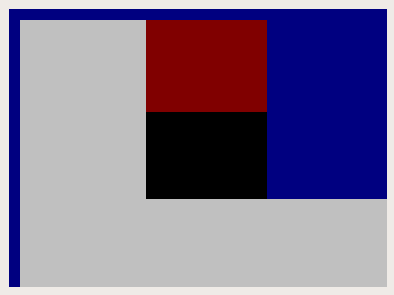
\includegraphics[width=0.4\textwidth]{situation_1_1}{}
\(\Rightarrow\)
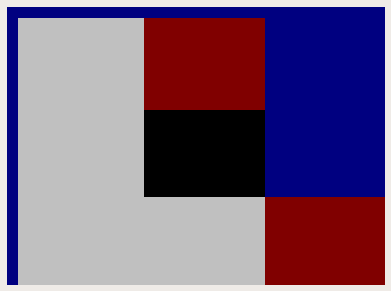
\includegraphics[width=0.4\textwidth]{situation_1_2}{}

Ici, il faut réagir tout de suite : deux pions bleus sont alignés et il y a de la place pour placer le troisième.
L'IA place donc tout simplement un pion rouge de telle sorte que le bleu ne puisse plus aligner trois pions.

\subsection{Situation 2}

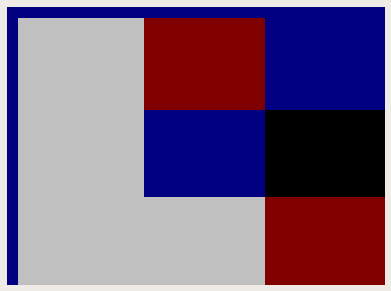
\includegraphics[width=0.4\textwidth]{situation_2_1}{}
\(\Rightarrow\)
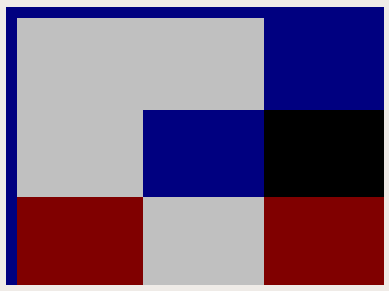
\includegraphics[width=0.4\textwidth]{situation_2_2}{}

Comme pour la situation précédente, le joueur bleu menace d'aligner trois pions, mais cette fois sur la diagonale.
L'IA se retrouve donc cette fois encore contrainte de bloquer le bleu. Elle réagit en déplaçant un pion rouge déjà en
place. À priori, il est plus efficace de toujours placer un nouveau pion tant qu'on en a un de disponible, mais l'arbre
de jeu n'est que de profondeur 3 et cette composante n'est pas prise en compte dans l'heuristique « normal ». Les coups « placer
un nouveau pion » et « déplacer le pion déjà existant » ont donc le même score (car dans tous les cas, cela ne permet pas
d'avoir plus de pions adjacents) et peuvent être tous les deux choisis aléatoirement.

\subsection{Situation 3}

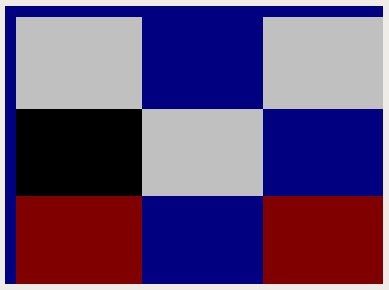
\includegraphics[width=0.4\textwidth]{situation_3_1}{}
\(\Rightarrow\)
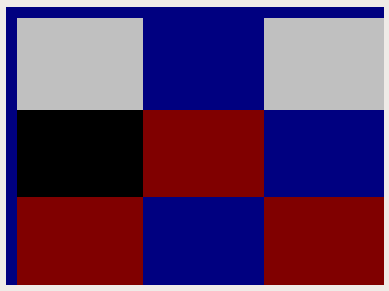
\includegraphics[width=0.4\textwidth]{situation_3_2}{}

Un peu plus tard dans la partie, cette situation survient. Le joueur rouge ne peut plus que perdre : soit il place un pion
rouge au centre et le bleu peut tout simplement faire un glissement de deux cases sur la gauche. Soit il fait un glissement
de la case grise sur la gauche et cela n'empêche toujours pas le bleu de faire un glissement, d'une seule case cette fois-ci, sur
la gauche. L'IA choisit donc l'une des meilleures solutions malgré sa défaite assurée : au cas où le joueur bleu fasse une erreur.

\section{Résultats}

Au fur et à mesure de l'implémentation des différents éléments de l'IA, nous avons obtenu divers résultats :

\begin{itemize}
    \item Nous avons découvert que le premier joueur a toujours moyen de gagner entre 4 et 6 coups
        (on a au début cru à une anomalie de l'algorithme nega-max).
    \item Il est aussi possible de tomber dans des cycles (ou états stables) où aucun joueur ne peut gagner.
    \item Nous avons pu classer les heuristiques selon le nombres de parties gagnées contre telle ou telle heuristiques à
        telle ou telle profondeur en faisant un mini tournoi d'IA\@. C'est là qu'on leur a donné leur nom « facile », « normal », …
    \item Il est aussi clair que l'IA est meilleure que le joueur à partir d'une certaine profondeur en particulier pour les
        heuristiques « difficile » et « légendaire ».
\end{itemize}

